
\section{Resultados}

Las estrategias de control implementadas fueron probadas con dos casos de prueba: bajo una referencia estática en un punto arbitrario y bajo el seguimiento de una trayectoria circular.

El caso bajo una referencia estática se evaluó el tiempo de estabilización y el error en estado estable y en el caso de seguimiento de trayectorias se evaluó qué tan robusto es el sistema y el comportamiento del mismo fuera del punto de linealización.

La trayectoria generada a seguir por la plataforma está definida por las siguientes ecuaciones:

\begin{equation} \label{equ: pos_tray}
    P = \begin{bmatrix}
    0.1 \cos (\omega t) \\
    0.1 \sen (\omega t) \\
    1.5
    \end{bmatrix}
\end{equation}

\begin{equation}\label{equ: vel_tray}
    \dot{P} = \begin{bmatrix}
    -0.1 \omega \sen (\omega t) \\
    0.1 \omega \cos (\omega t) \\
    0
    \end{bmatrix}
\end{equation}

Se planea hacer que la plataforma efectúe el recorrido en 10 segundos. 
La trayectoria describe un círculo de radio de $0.1 \ [m]$
por lo tanto  $\omega = \pi / 10 \ [rad/s]$. 
En la simulación de la trayectoria no se contemplan movimientos en los ángulos de alabeo, cabeceo y guiñada.

Los controles que fueron implementados generaron diferentes resultados en el movimiento y el punto final una vez que se estabilizó el sistema. 
Los resultados se presentan a continuación.

\subsection{Control PD}
En las figuras \ref{fig:PD position} y \ref{fig:PD error} se observa el comportamiento de la plataforma bajo control PD para una trayectoria de movimiento generada por las ecuaciones \ref{equ: pos_tray} y \ref{equ: vel_tray}. 
En la figura \ref{fig:PD error} se observa la presencia de un error que que el sistema es incapaz de eliminar sin importar que la plataforma sigue los puntos de la trayectoria generada.

En las figuras \ref{fig:PD positione} y \ref{fig:PD errore} se observa el comportamiento de la plataforma bajo control PD para una referencia estática. 
Observando la figura \ref{fig:PD errore} se visualiza que existe un error constante en los ejes X, Y y Z. 
Este error es similar al error del caso anterior, puesto que el control PD no tiene manera de corregir el error en el estado estable.


\begin{figure}[H]
    \centering
    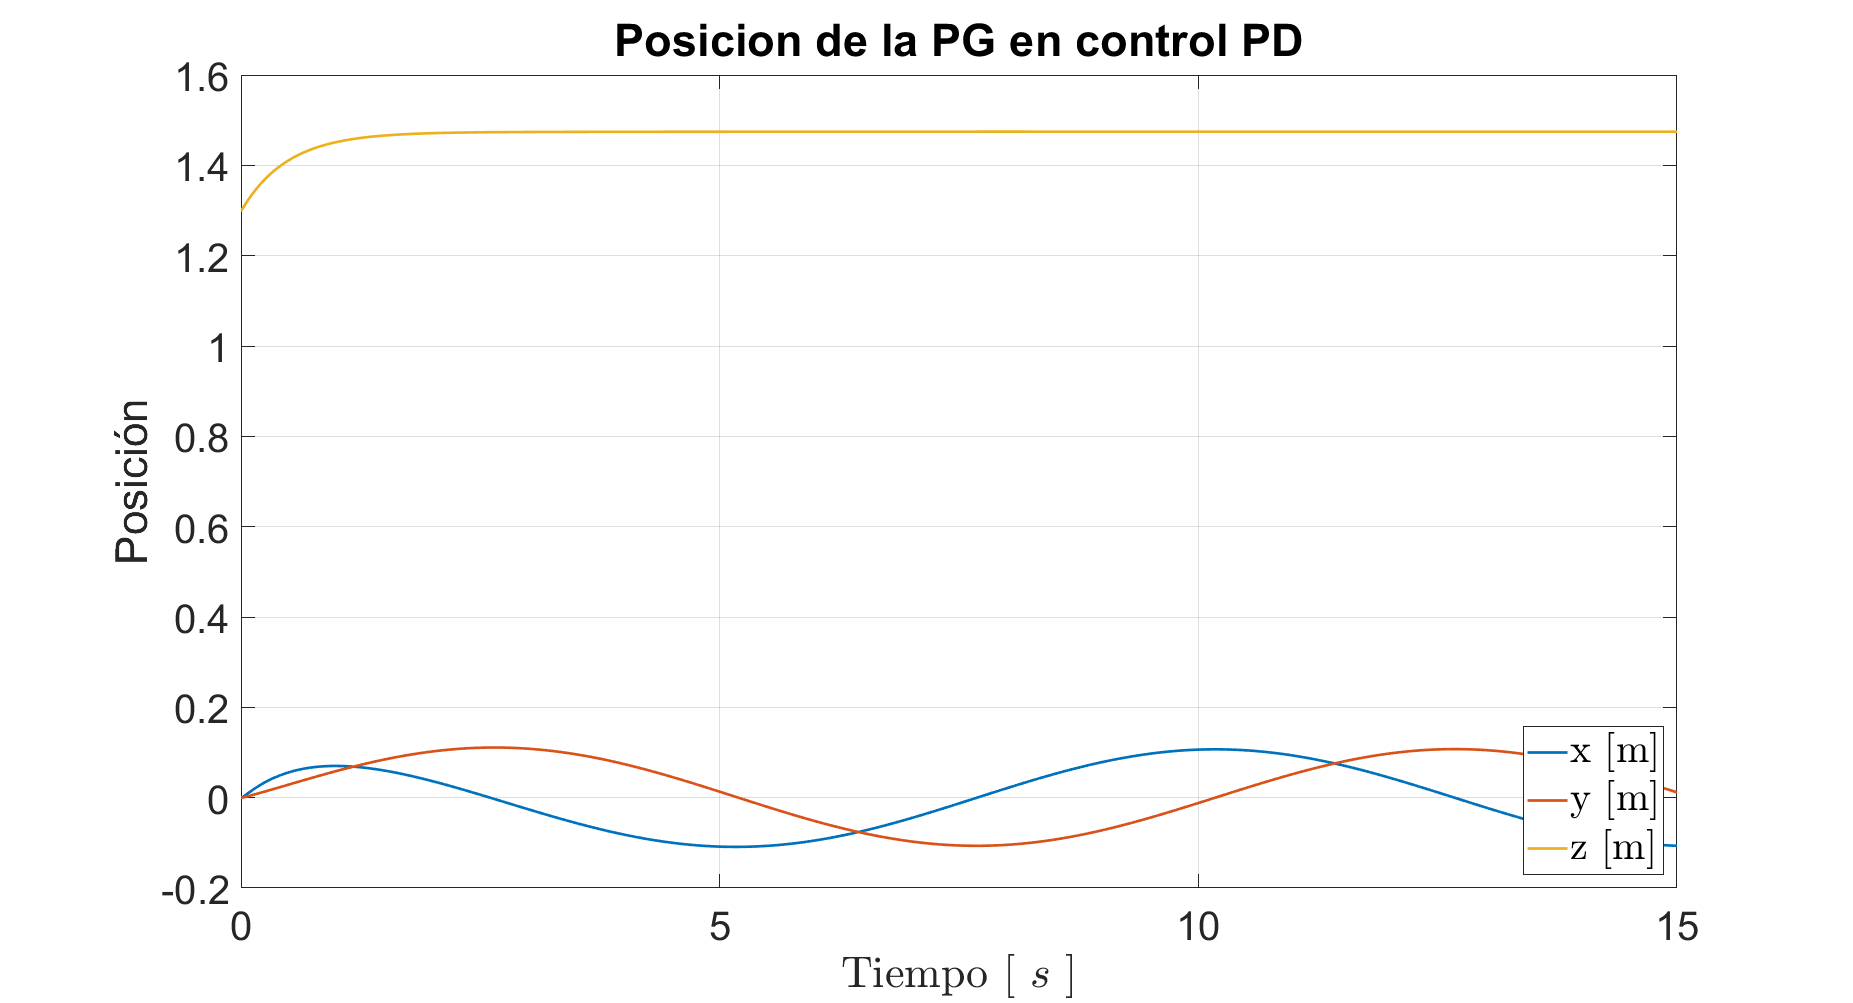
\includegraphics[width=0.4\textwidth]{posPD.png}
    \caption{Posición del sistema bajo un patrón de movimiento - PD.}
    \label{fig:PD position}
\end{figure}

\begin{figure}[H]
    \centering
    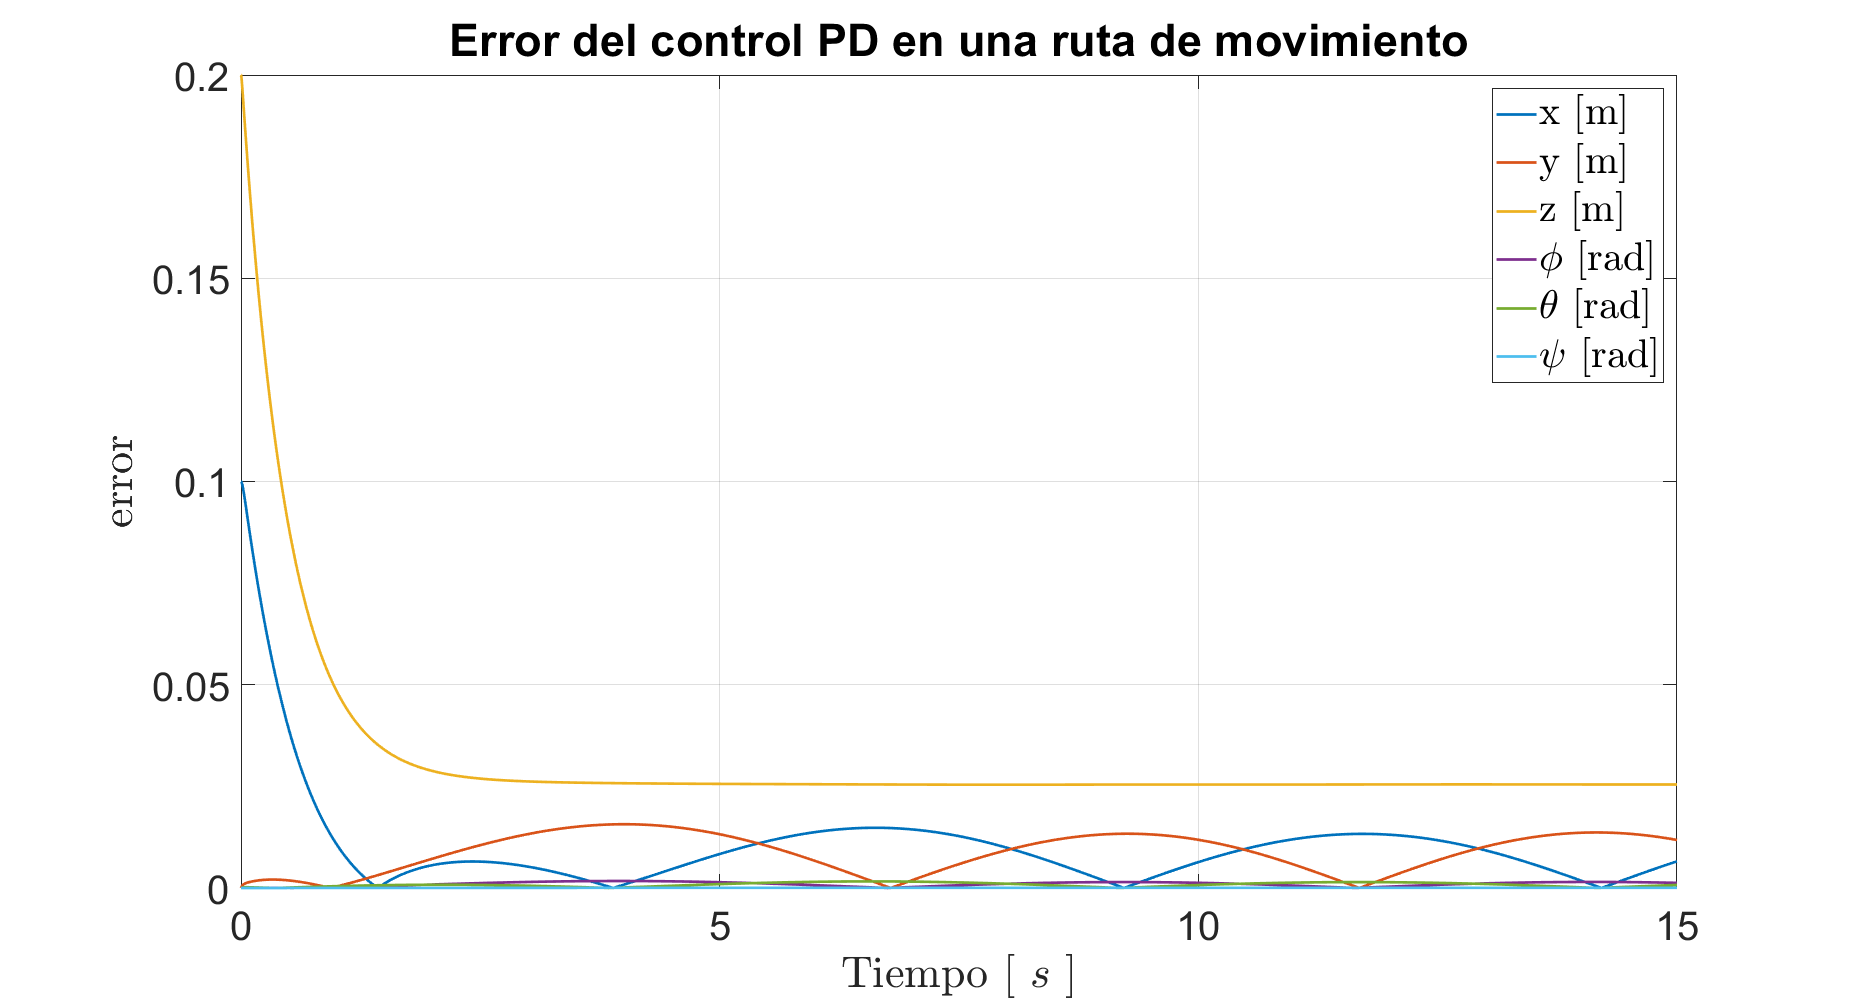
\includegraphics[width=0.4\textwidth]{errorPD.png}
    \caption{Error del sistema bajo un patrón de movimiento- PD.}
    \label{fig:PD error}
\end{figure}

\begin{figure}[H]
    \centering
    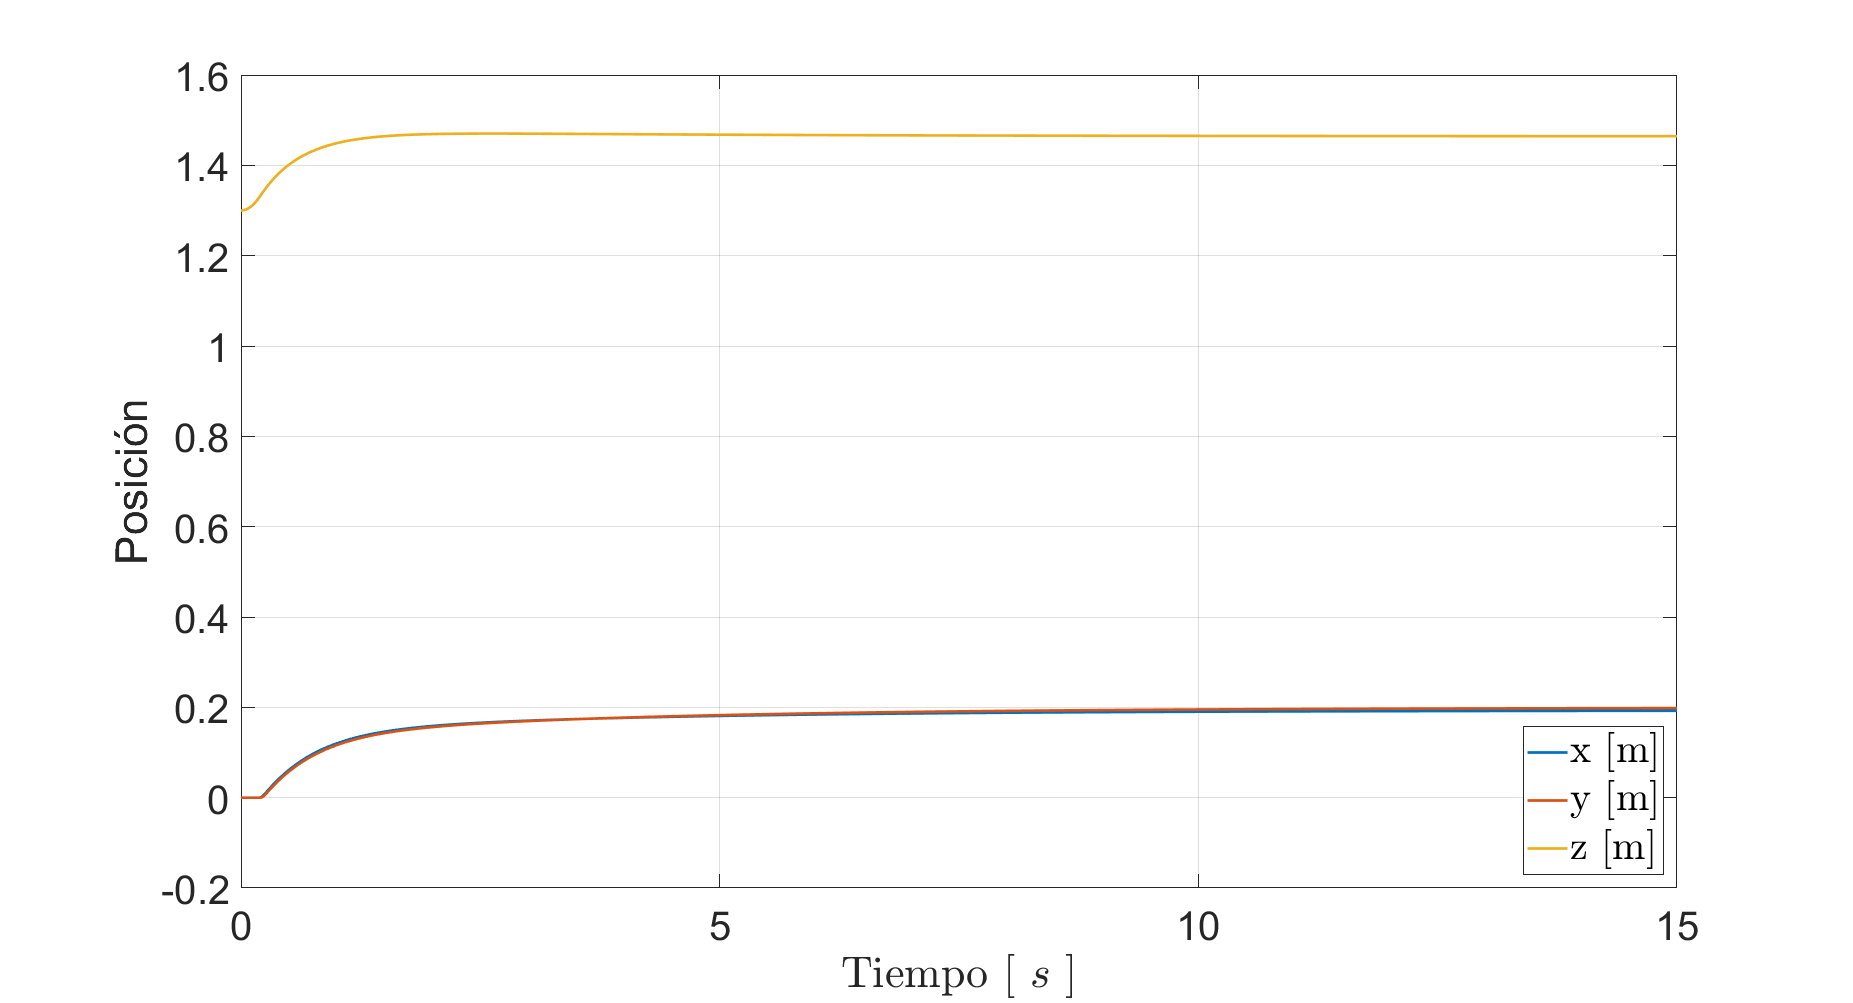
\includegraphics[width=0.4\textwidth]{posPDe.png}
    \caption{Posición del sistema bajo una referencia estática- PD.}
    \label{fig:PD positione}
\end{figure}

\begin{figure}[H]
    \centering
    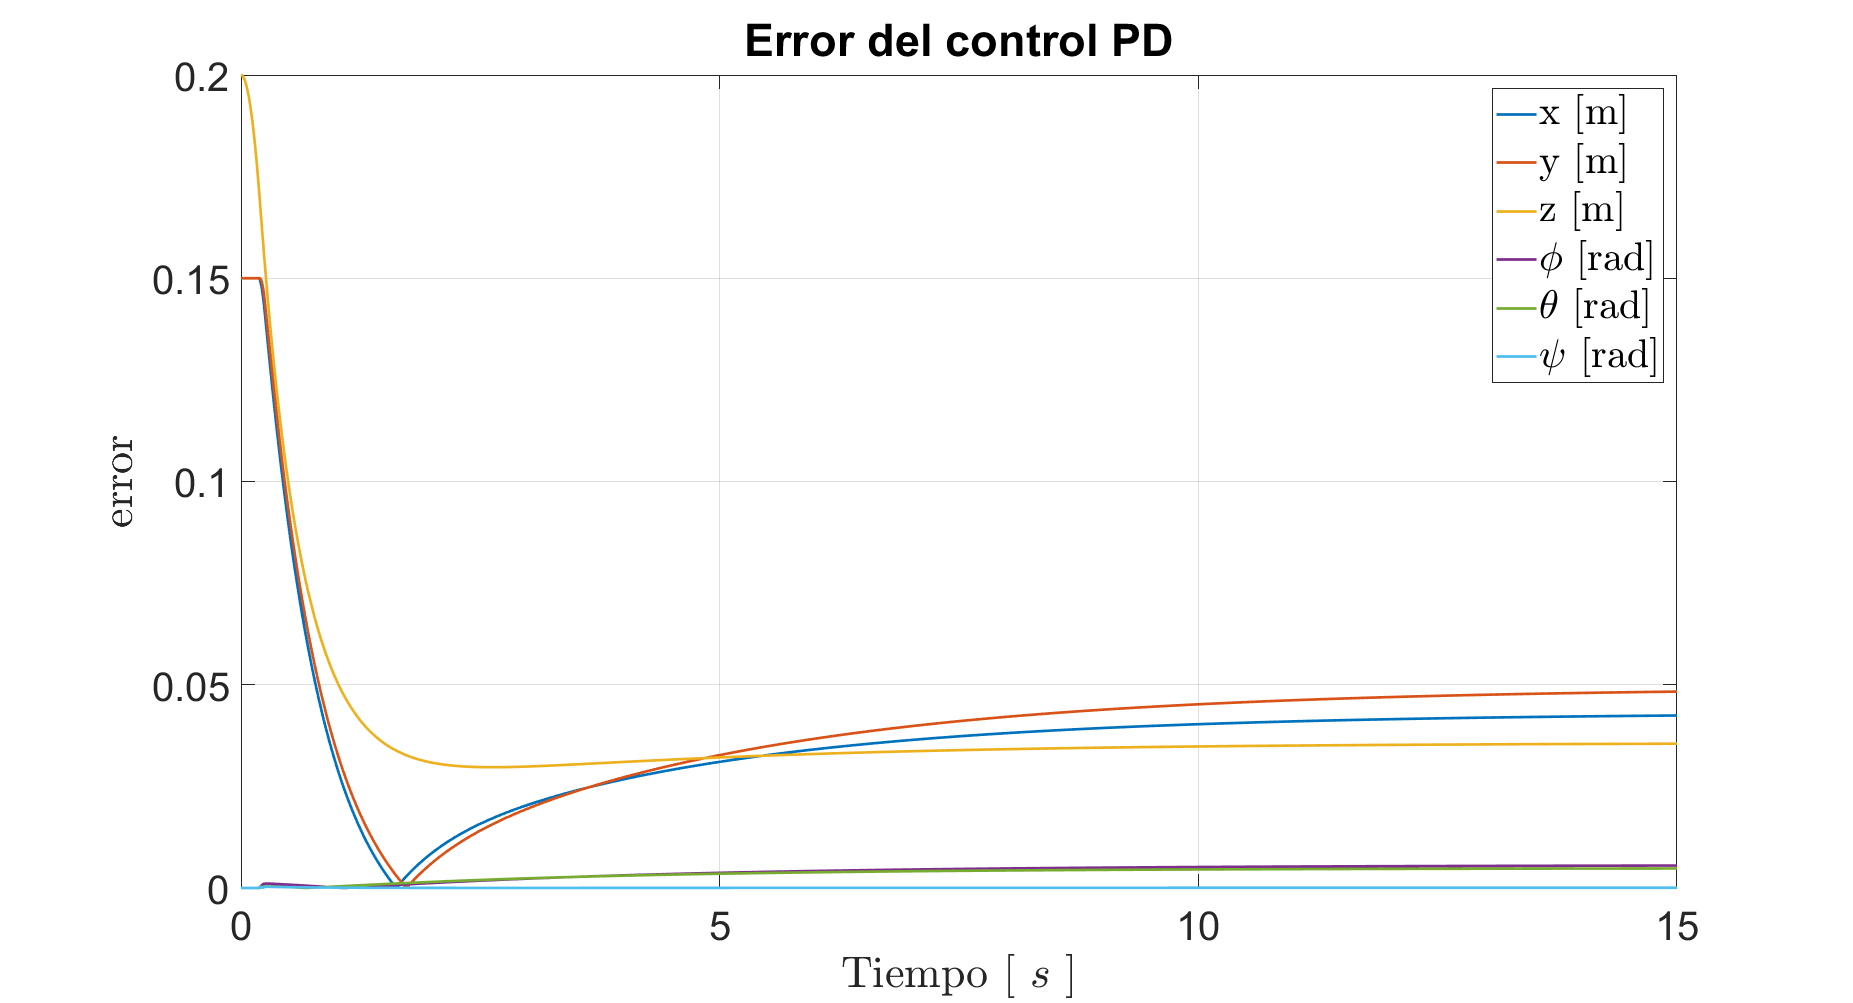
\includegraphics[width=0.4\textwidth]{errorPDe.png}
    \caption{Error del sistema bajo una referencia estática - PD.}
    \label{fig:PD errore}
\end{figure}



\subsection{Control PD+G}

En las figuras \ref{fig:PDG position} y \ref{fig:PDG error} se observa el comportamiento de la plataforma bajo control PD + G en la trayectoria de movimiento generada por las ecuaciones \ref{equ: pos_tray} y \ref{equ: vel_tray}. 
A diferencia del control PD, el control PD + G es capaz de reducir el error estacionario de la plataforma. 
No obstante debido al cálculo de las ganancias del controlador para un punto de linealización diferente a los puntos de la trayectoria,
la plataforma sigue experimentando un error en estado estable debido al comportamiento no linear del sistema real.

En las figuras \ref{fig:PDG positione} y \ref{fig:PDG errore} se observa el comportamiento de la plataforma bajo control PD + G en una referencia estática. 
Al igual que en el caso de patrón de movimiento, la plataforma se acerca a la referencia más que con el control PD. 
El cálculo de ganancias del controlador para una posición específica
produce un error nuevamente ya que el punto de linealización es diferente a la posición deseada.


\begin{figure}[H]
    \centering
    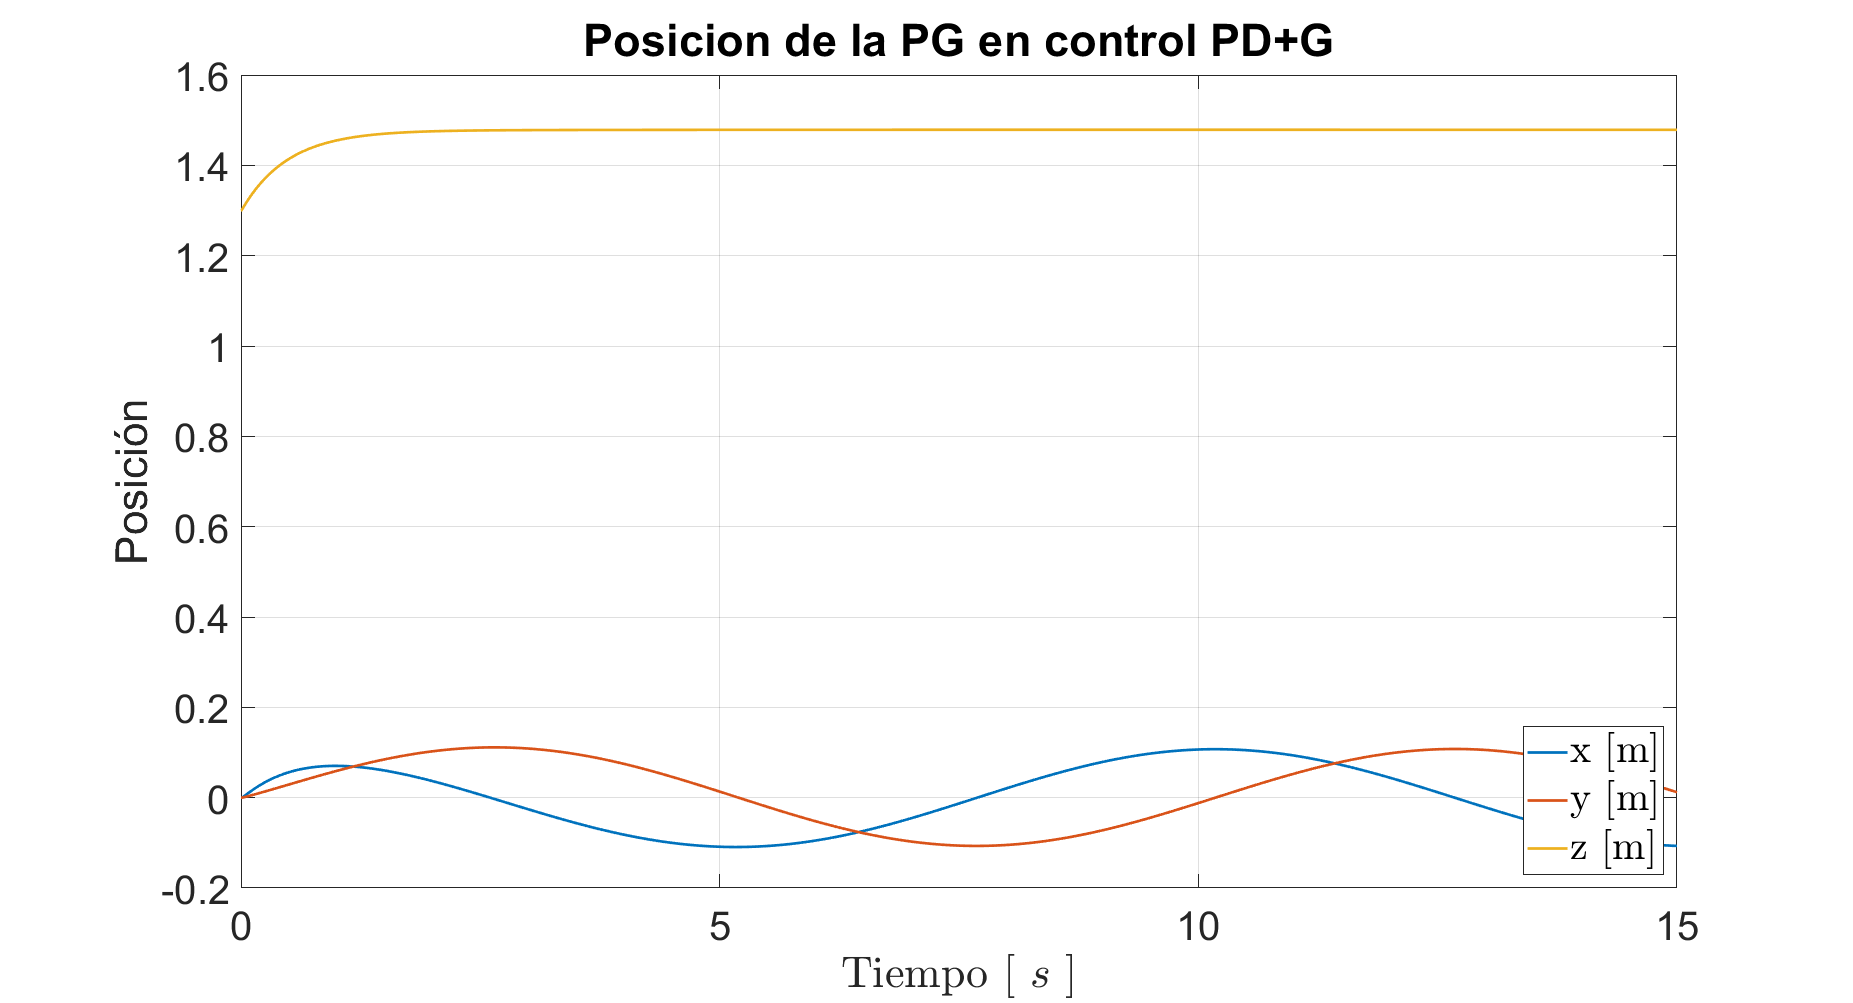
\includegraphics[width=0.4\textwidth]{posPDpG.png}
    \caption{Posición del sistema bajo un patrón de movimiento - PD+G.}
    \label{fig:PDG position}
\end{figure}

\begin{figure}[H]
    \centering
    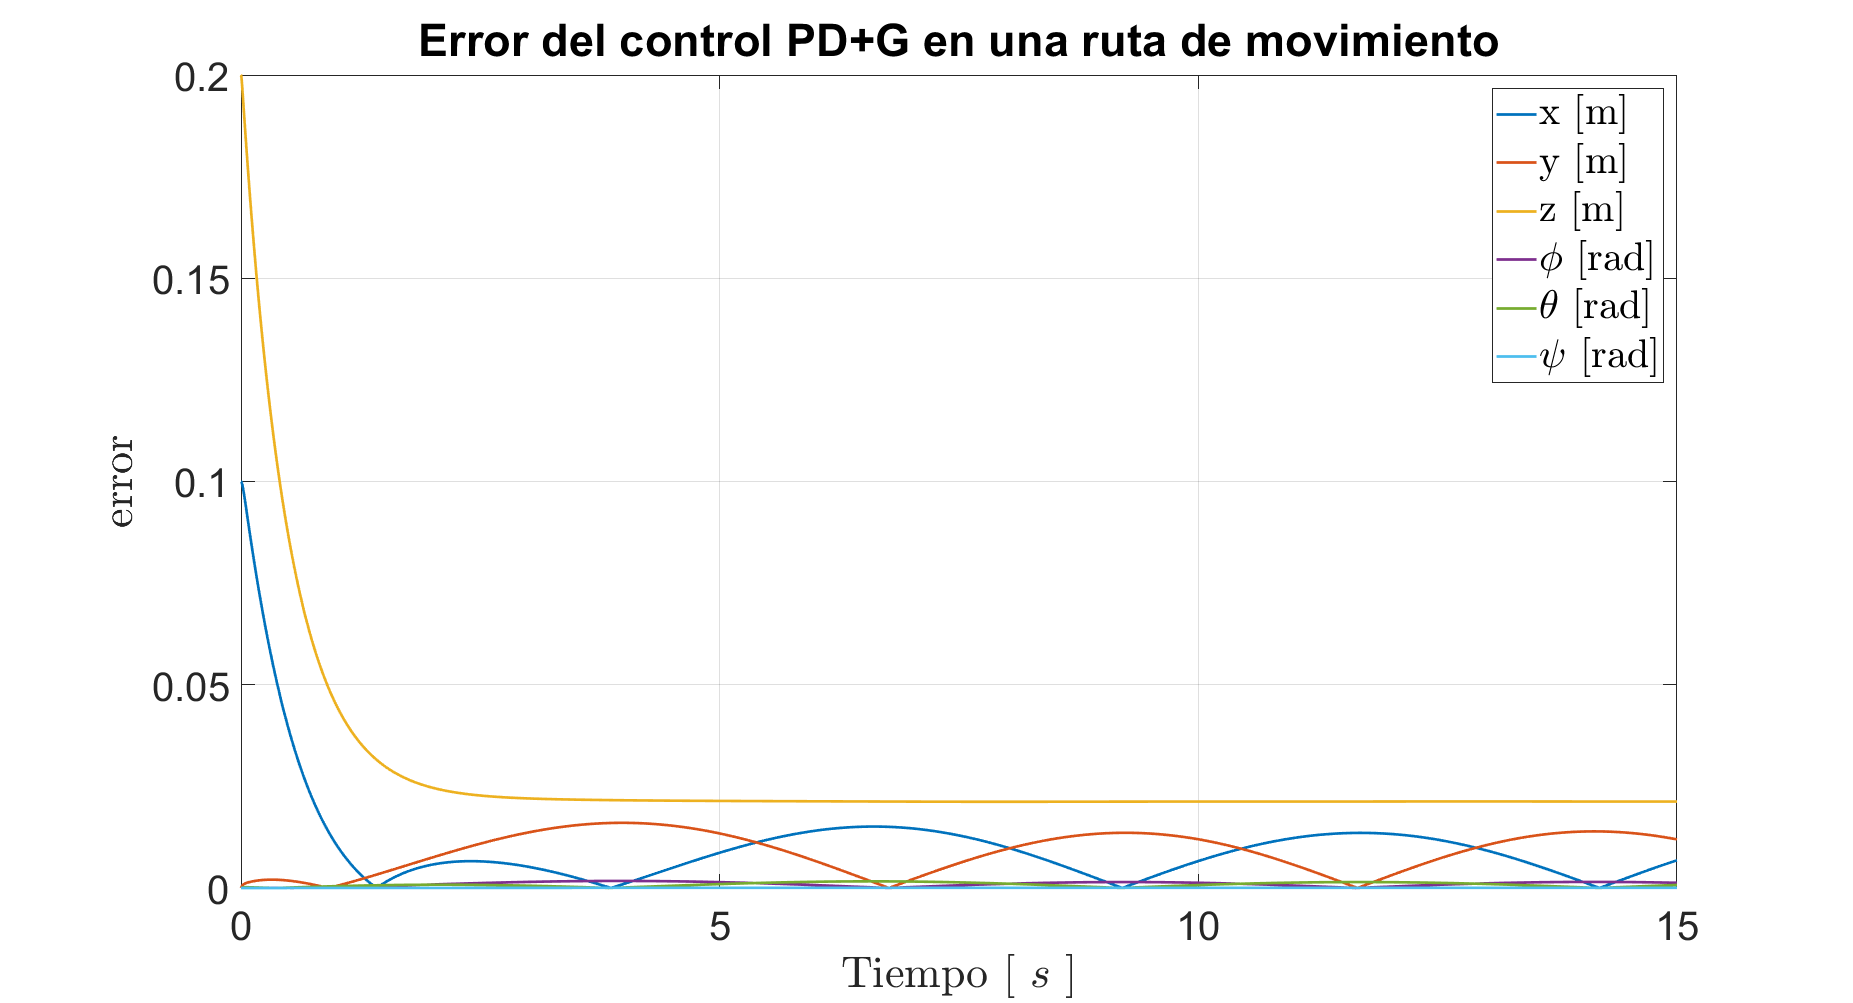
\includegraphics[width=0.4\textwidth]{errorPDpG.png}
    \caption{Error del sistema bajo un patrón de movimiento - PD+G.}
    \label{fig:PDG error}
\end{figure}

\begin{figure}[H]
    \centering
    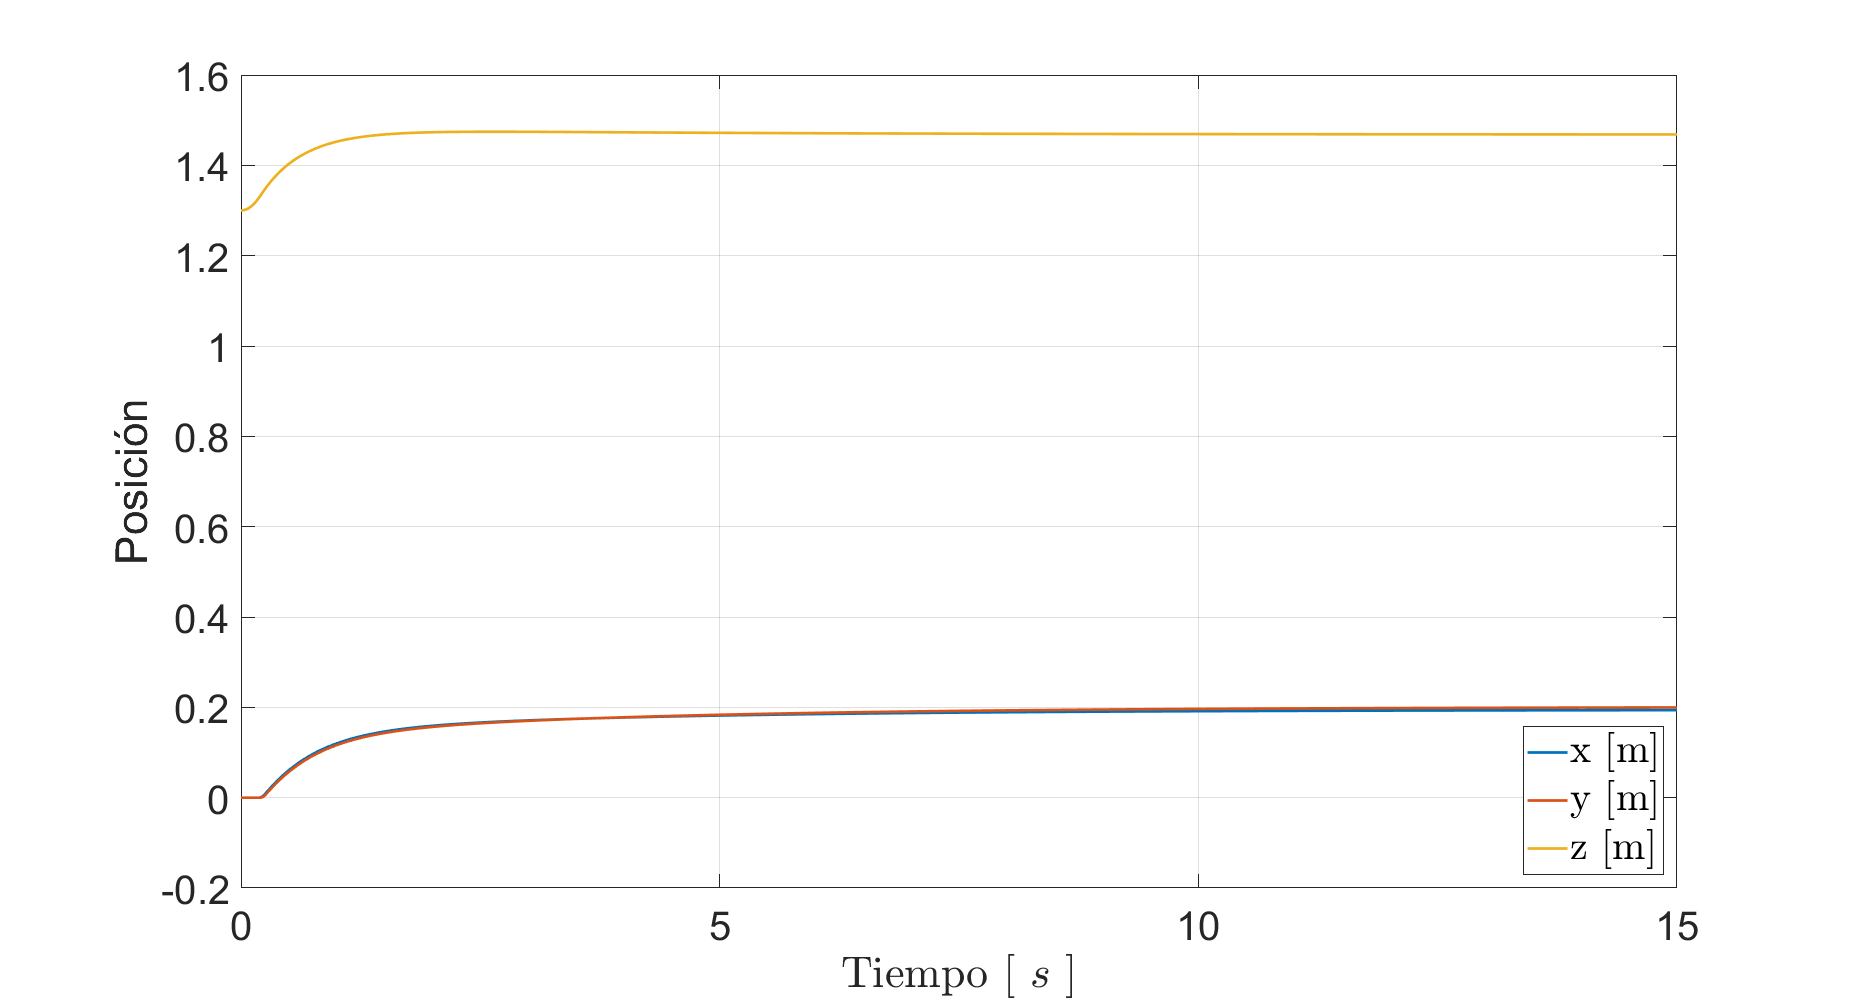
\includegraphics[width=0.4\textwidth]{posPDpGe.png}
    \caption{Posición del sistema bajo una referencia estática - PD+G.}
    \label{fig:PDG positione}
\end{figure}

\begin{figure}[H]
    \centering
    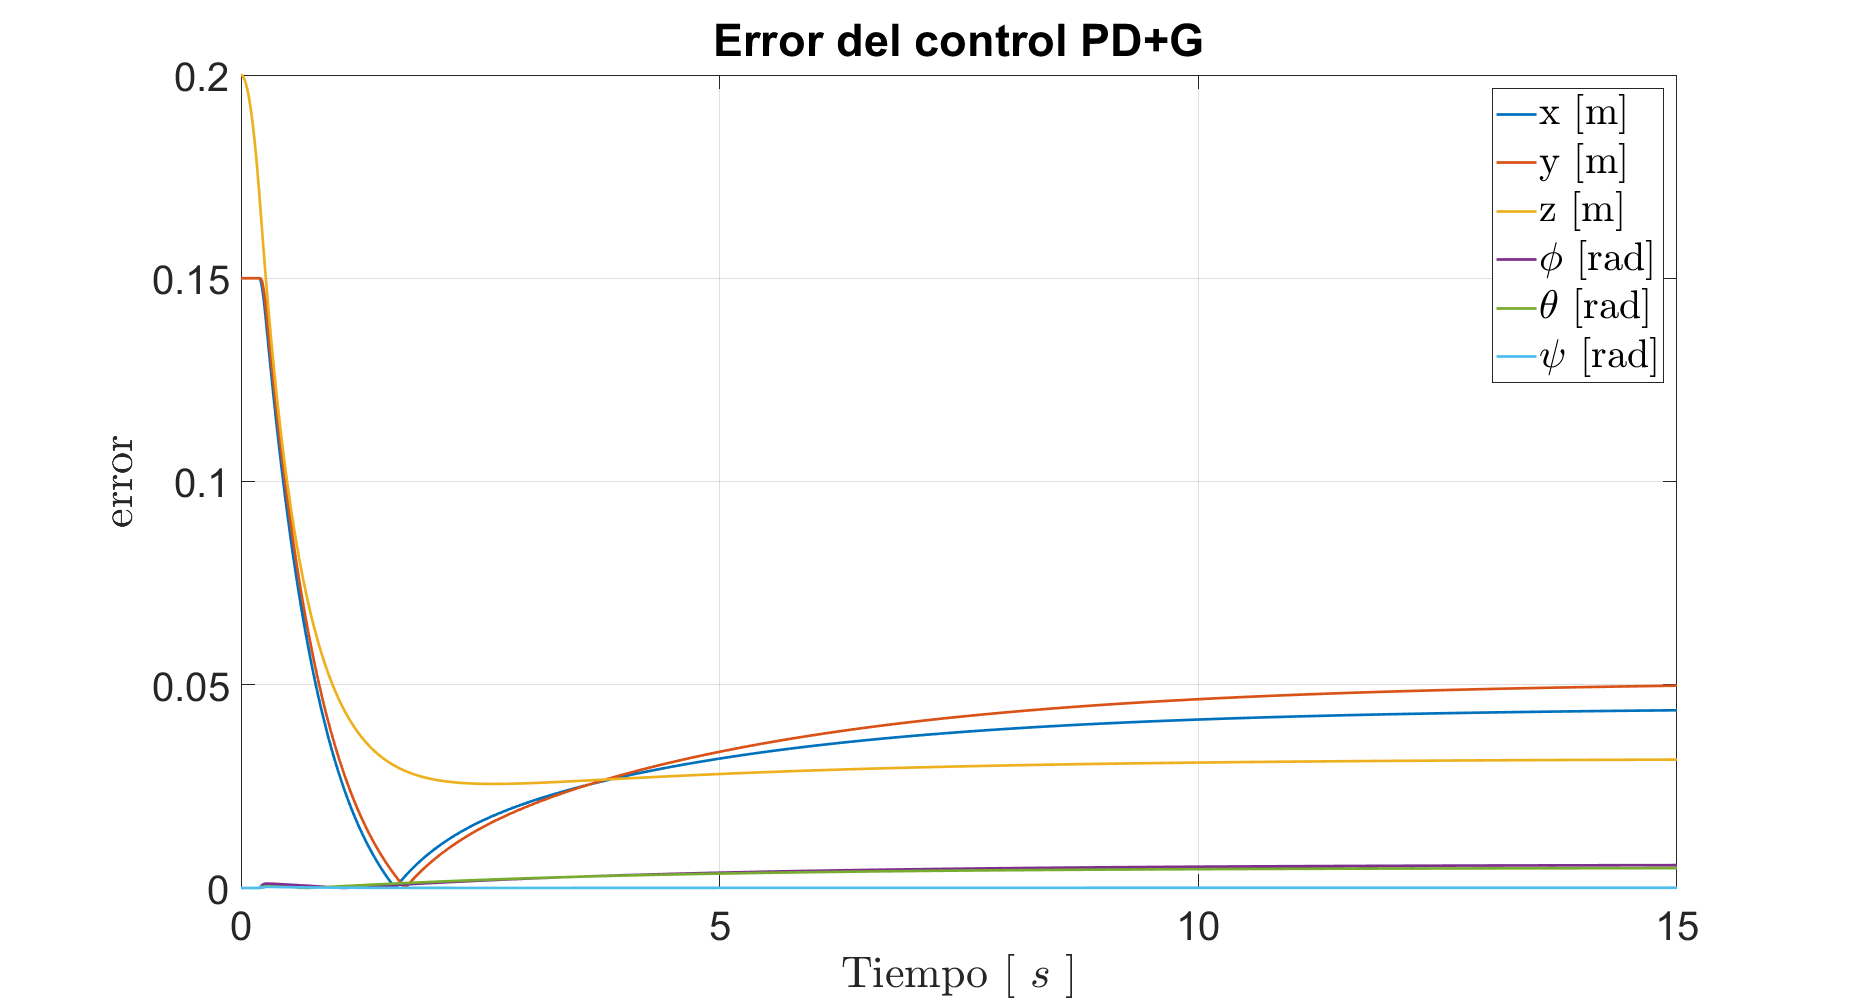
\includegraphics[width=0.4\textwidth]{errorPDpGe.png}
    \caption{Error del sistema bajo una referencia estática - PD+G.}
    \label{fig:PDG errore}
\end{figure}



\subsection{Control PID}
En las figuras \ref{fig:PID position} y \ref{fig:PID error} se observa el comportamiento de la plataforma bajo control PID en la trayectoria generada por las ecuaciones \ref{equ: pos_tray} y \ref{equ: vel_tray}.
A diferencia de los controles anteriores (PD y PD + G), el control PID es capaz de eliminar el error en estado estable debido al efecto
de la integración. 
La figura \ref{fig:PID error} muestra cómo el error durante el movimiento se acerca constantemente a cero.

En las figuras \ref{fig:PID positione} y \ref{fig:PID errore} se observa el comportamiento de la plataformas bajo control PID en una referencia estática. 
Se observa que el error en estado estable se reduce de manera similar al caso del patrón de movimiento.
Sin embargo, aún conserva un error debido al tiempo de simulación. 
Al incrementar éste valor, el error se reducirá hasta ser eliminado.

\begin{figure}[H]
    \centering
    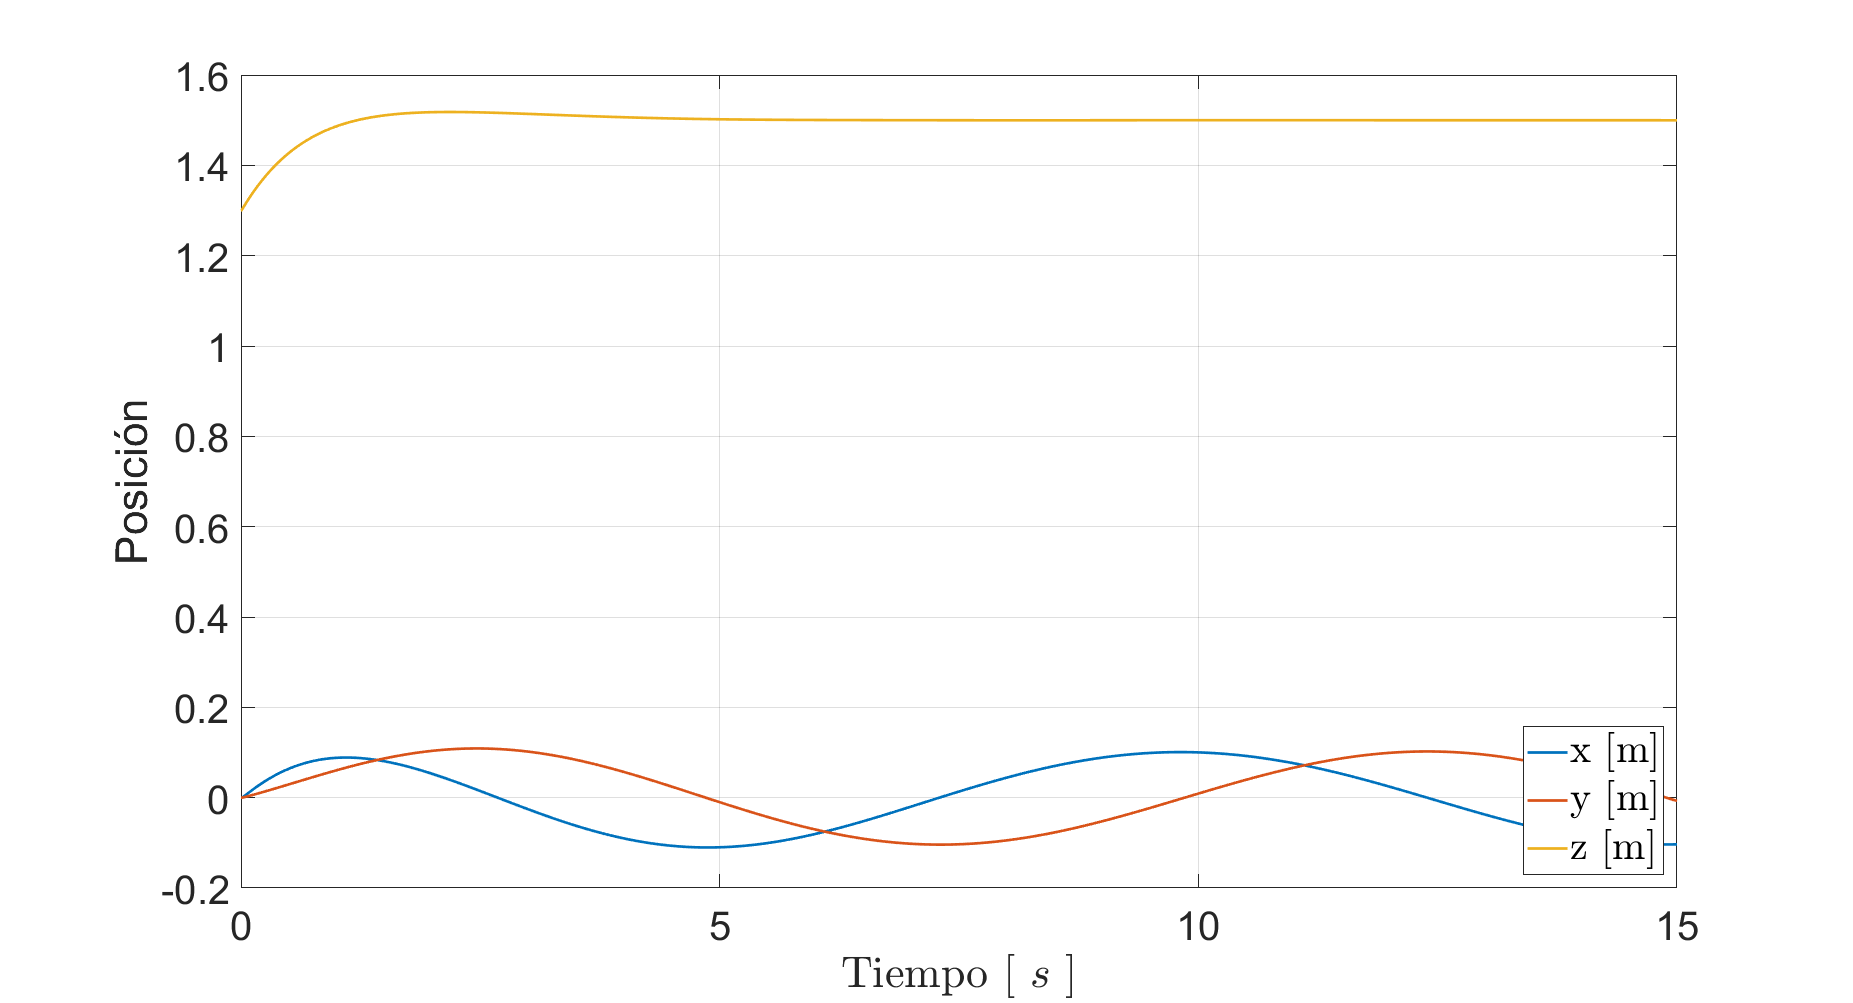
\includegraphics[width=0.4\textwidth]{posPID.png}
    \caption{Posición del sistema bajo un patrón de movimiento - PID.}
    \label{fig:PID position}
\end{figure}

\begin{figure}[H]
    \centering
    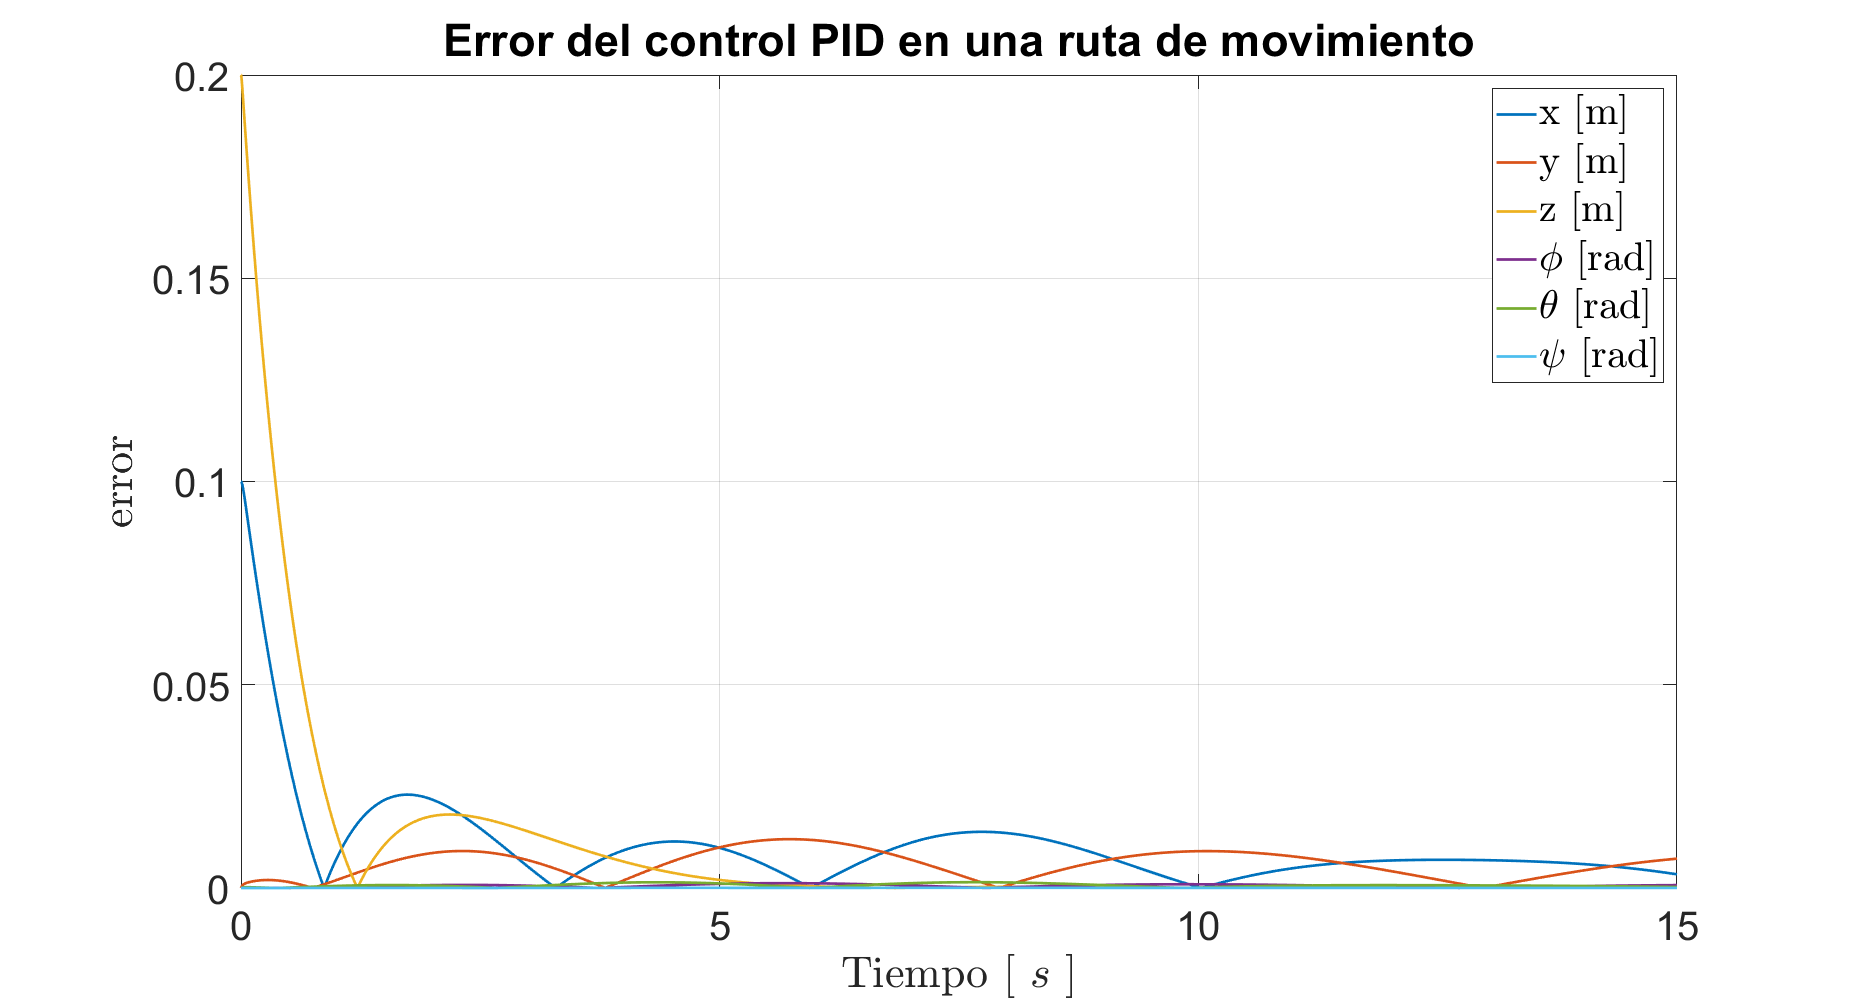
\includegraphics[width=0.4\textwidth]{errorPID.png}
    \caption{Error del sistema bajo un patrón de movimiento - PID.}
    \label{fig:PID error}
\end{figure}

\begin{figure}[H]
    \centering
    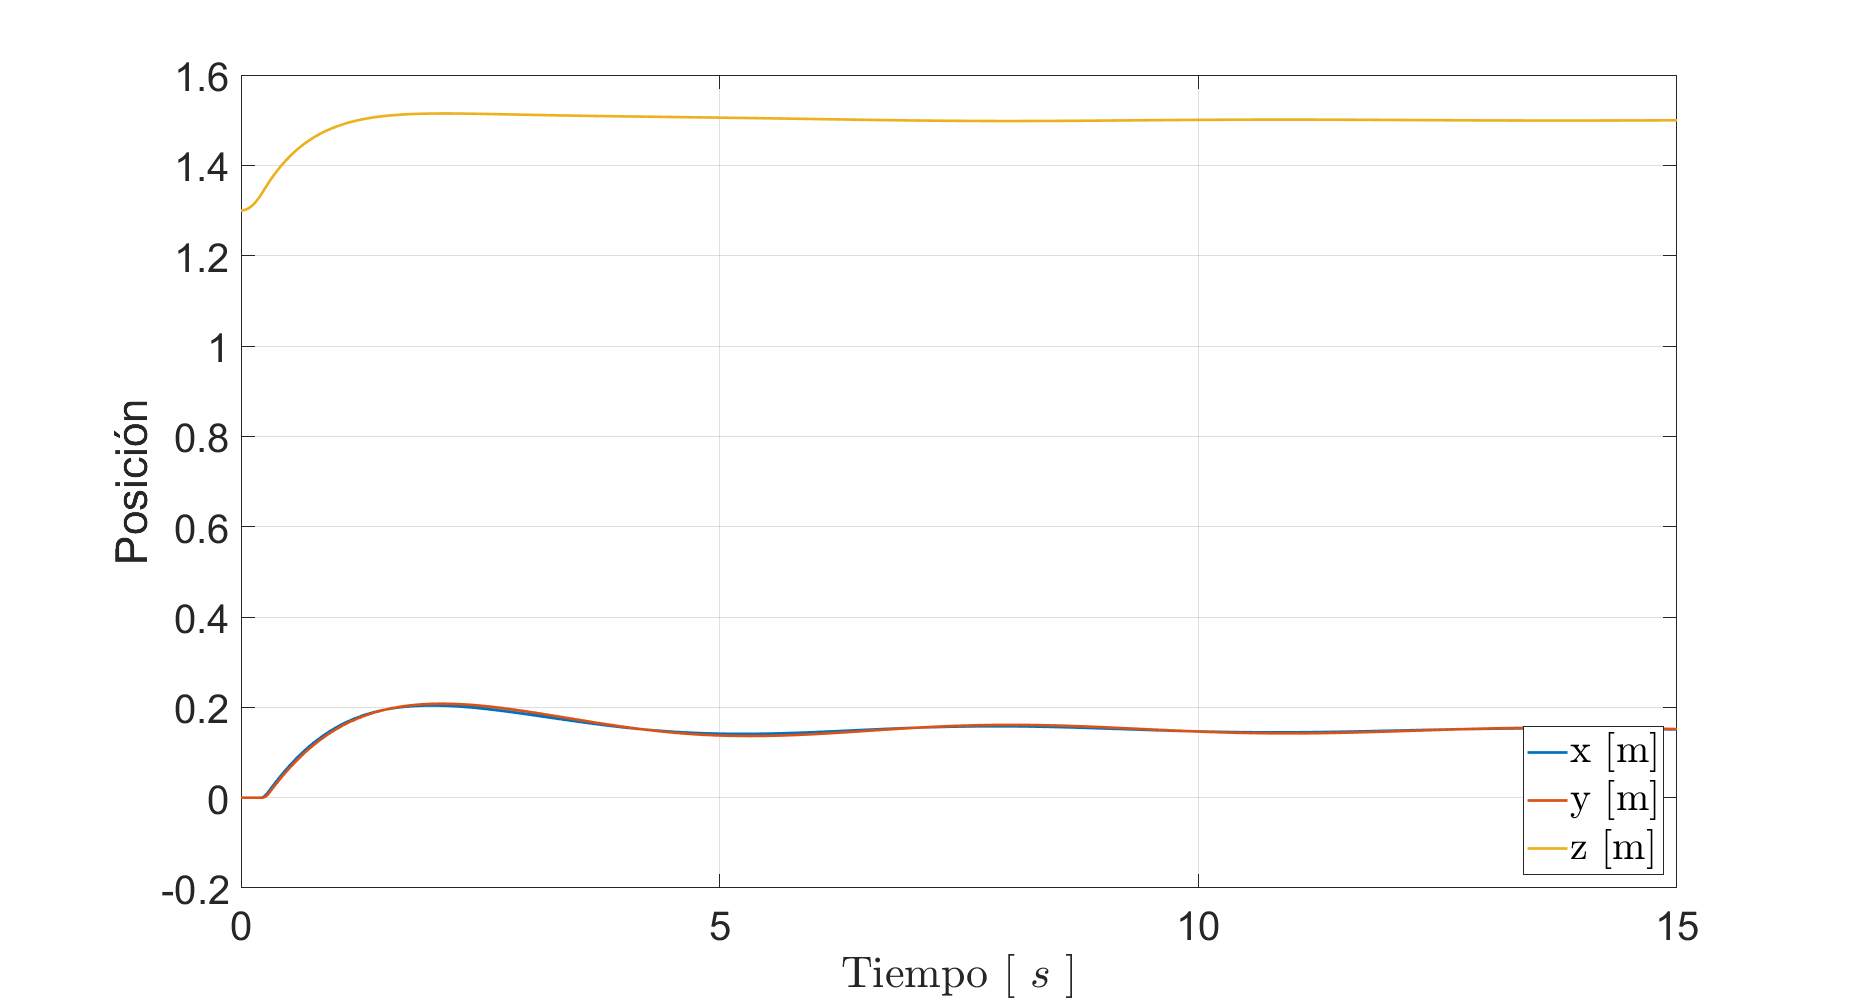
\includegraphics[width=0.4\textwidth]{posPIDe.png}
    \caption{Posición del sistema bajo una referencia estática - PID.}
    \label{fig:PID positione}
\end{figure}

\begin{figure}[H]
    \centering
    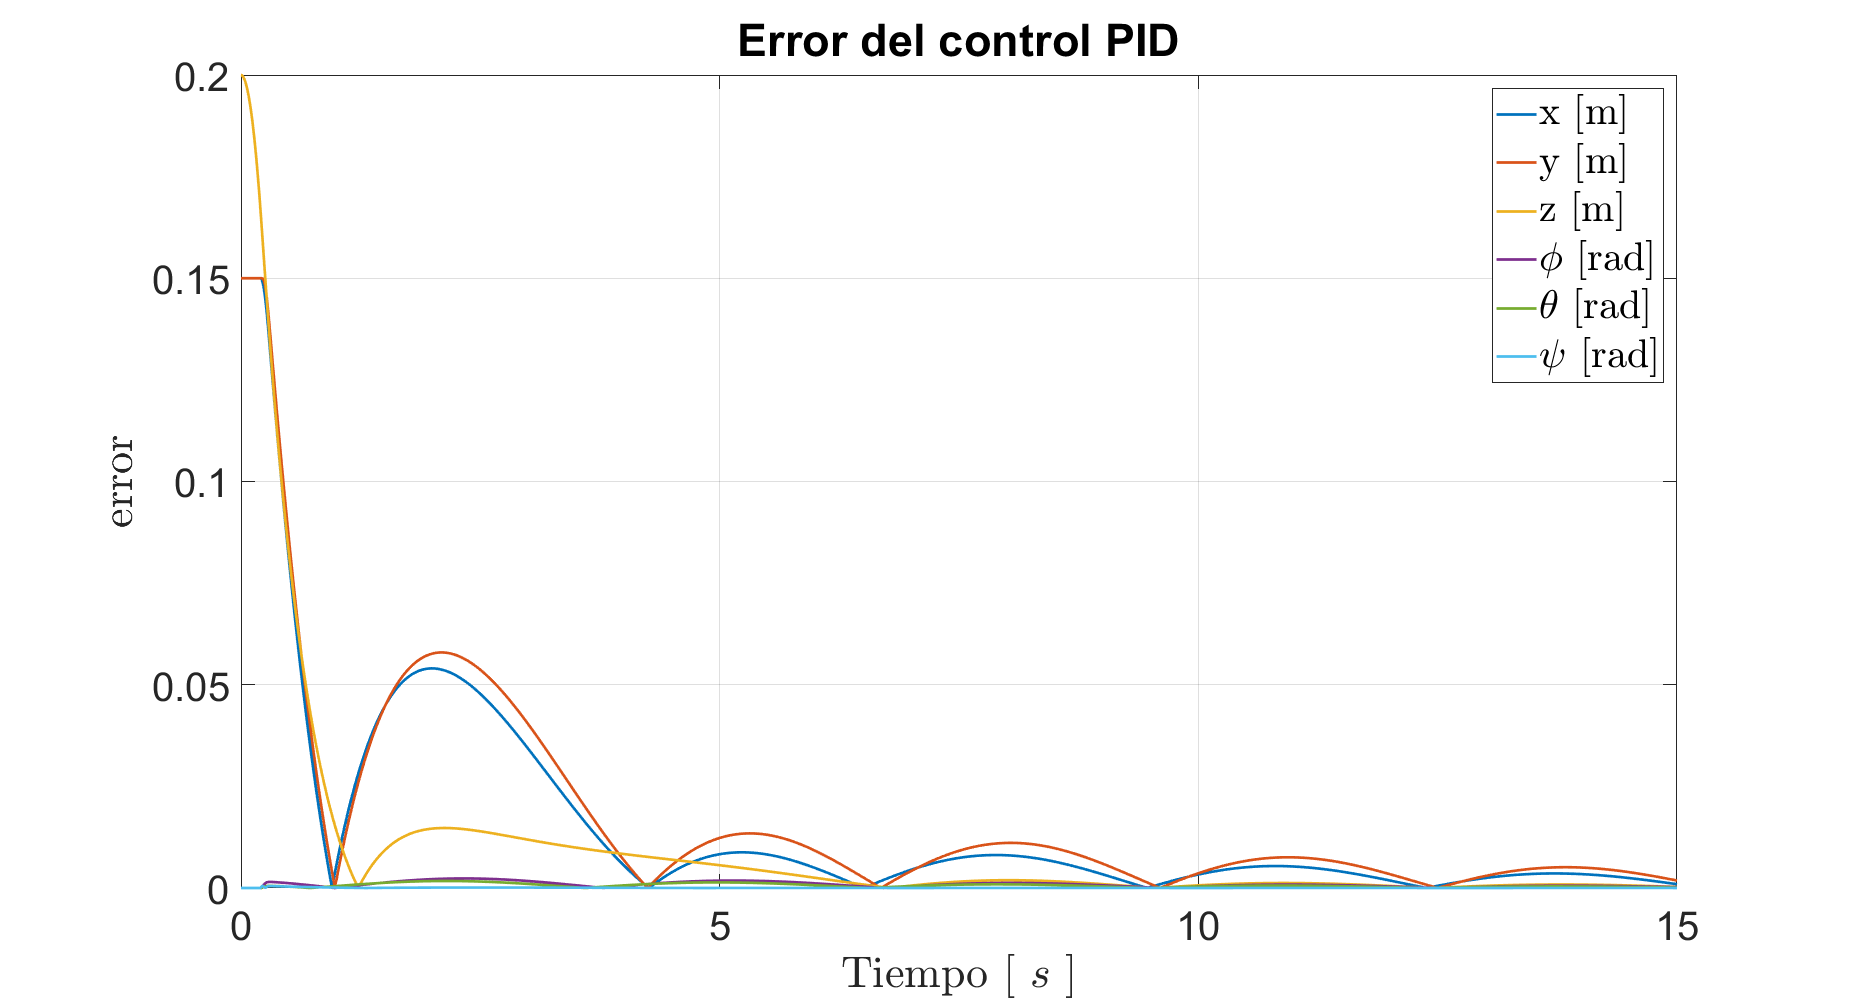
\includegraphics[width=0.4\textwidth]{errorPIDe.png}
    \caption{Error del sistema bajo una referencia estática - PID.}
    \label{fig:PID errore}
\end{figure}



\subsection{Trabajo}

En las figuras \ref{fig:energiamov} y \ref{fig:energiaest} se observan las comparaciones energéticas de los tres controles en las misma tareas. 

\begin{itemize}
    \item La trayectoria que debe ser recorrida por el robot está dada por las ecuaciones \ref{equ: pos_tray} y \ref{equ: vel_tray}.
    \item El movimiento a una referencia estática. 
\end{itemize}

\begin{figure}[H]
    \centering
    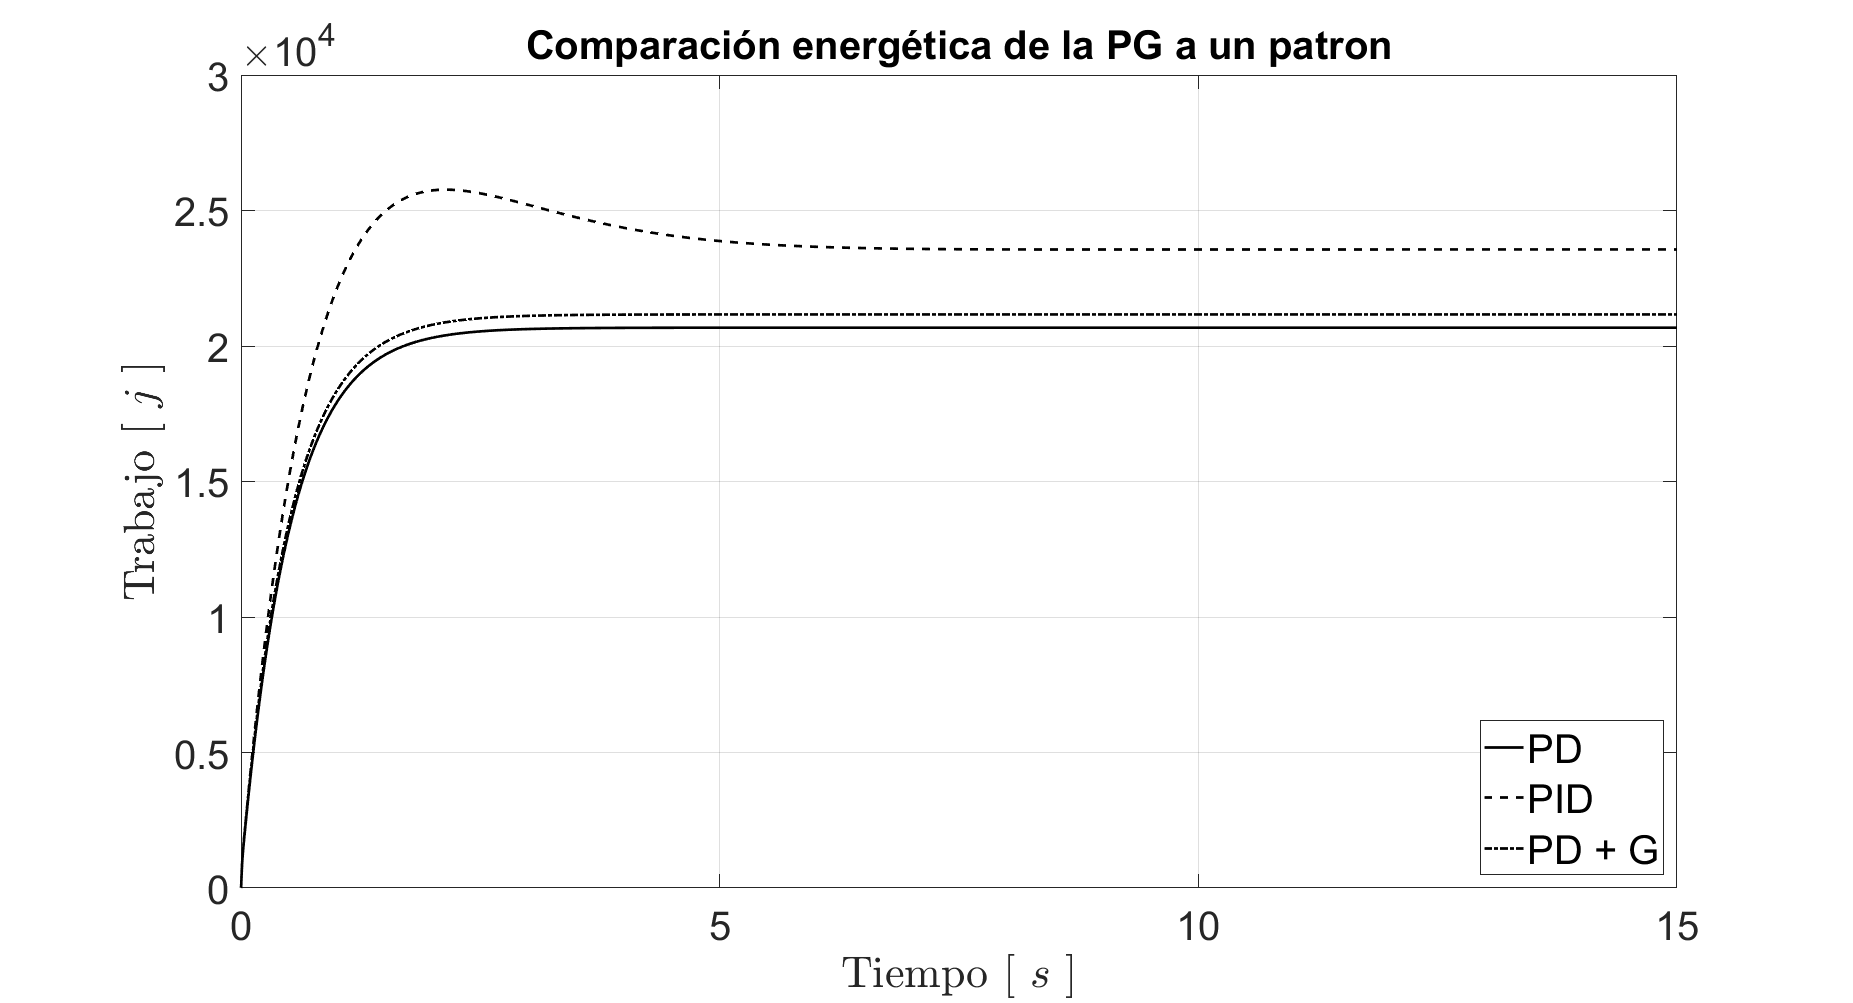
\includegraphics[width=0.4\textwidth]{energiamov.png}
    \caption{Comparación de energía en los diferente controles bajo un patrón de movimiento.}
    \label{fig:energiamov}
\end{figure}

\begin{figure}[H]
    \centering
    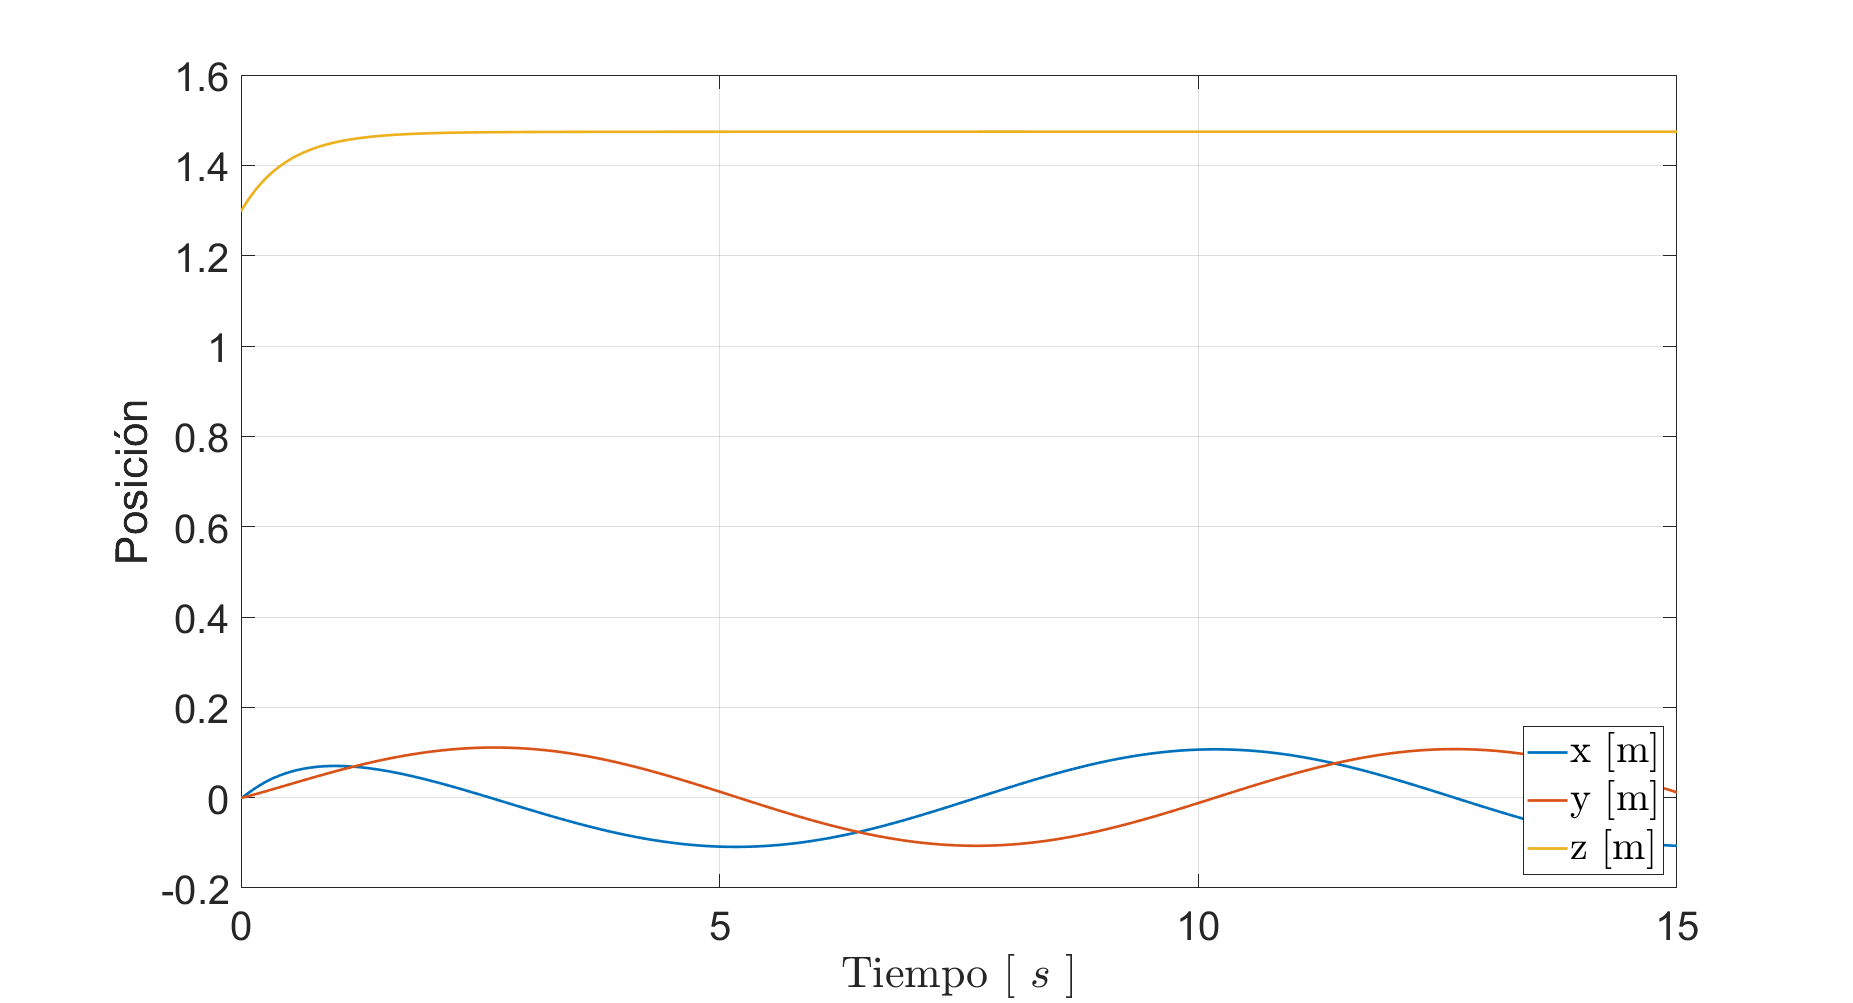
\includegraphics[width=0.4\textwidth]{Energiaestatica.png}
    \caption{Comparación de energía en los diferente controles bajo referencia constante.}
    \label{fig:energiaest}
\end{figure}

Para ambos casos la siguiente relación de gasto energético se preserva:

\begin{equation}
    PID > PD + G > PD
\end{equation}

El consumo energético del cotrol PID es mayor a las otras dos estrategias debido a la naturaleza del controlador.
El componente de integración obliga al sistema a consumir más energía, siendo capaz de presentar un sobretiro en su movimiento.
No obstante, este incremente en el consumo energético trae consigo la ventaja de poseer el error en estado estable mínimo de las estrategias de control evaluadas.


En cuanto al error, los controles en ambos casos siguen el siguiente patrón:

\begin{equation}
    PD > PD + G > PID
\end{equation}